\documentclass[aspectratio=169,xcolor={dvipsnames}]{beamer}
\usetheme{Madrid}
\usecolortheme{default}

% Packages
\usepackage{graphicx}
\usepackage{booktabs}
\usepackage{amsmath}
\usepackage{siunitx}
\usepackage{tikz}
\usepackage{pgfplots}
\pgfplotsset{compat=1.18}

% Custom colors (IEEE-like blue)
\definecolor{ieeeblue}{RGB}{0,102,204}
\setbeamercolor{structure}{fg=ieeeblue}
\setbeamercolor{title}{fg=white,bg=ieeeblue}
\setbeamercolor{frametitle}{fg=white,bg=ieeeblue}

% Macros
\newcommand{\rmse}{\ensuremath{\mathrm{RMSE}}}
\newcommand{\rTwo}{\ensuremath{\mathrm{R}^2}}
\newcommand{\da}{\ensuremath{\mathrm{DA}}}

% Font size settings
\setbeamerfont{title}{size=\Large}
\setbeamerfont{frametitle}{size=\large}
\setbeamerfont{normal text}{size=\normalsize}

% Remove navigation symbols
\setbeamertemplate{navigation symbols}{}

% Footer
\setbeamertemplate{footline}[frame number]

% Title information
\title[Multi-Horizon Stock Prediction]{Benchmarking Transformers and Baselines\\for Multi-Horizon Stock Return Prediction}
\subtitle{Technical and Earnings Features on the Dow 30}
\author[Siu \& Chan]{Nelson Siu\inst{1} \and Jonathan H. Chan\inst{2}}
\institute[UofT \& KMUTT]{
  \inst{1}Division of Engineering Science, University of Toronto\\
  \inst{2}Innovative Cognitive Computing, King Mongkut's University of Technology Thonburi
}
\date{IEEE Conference 2025}

\begin{document}

% ============================================
% TITLE SLIDE
% ============================================
\begin{frame}
  \titlepage
\end{frame}

% ============================================
% OUTLINE
% ============================================
\begin{frame}{Outline}
  \tableofcontents
\end{frame}

% ============================================
% SECTION 1: INTRODUCTION
% ============================================
\section{Introduction \& Motivation}

\begin{frame}{The Challenge: Multi-Horizon Stock Prediction}
  \begin{columns}[T]
    \begin{column}{0.55\textwidth}
      \textbf{Why is this hard?}
      \begin{itemize}
        \item Noisy, low signal-to-noise ratio
        \item Regime-dependent patterns
        \item Market efficiency limits
        \item Non-stationarity
      \end{itemize}
      
      \vspace{0.5cm}
      \textbf{Why does it matter?}
      \begin{itemize}
        \item Trading strategies
        \item Risk management
        \item Portfolio optimization
        \item Understanding market dynamics
      \end{itemize}
    \end{column}
    
    \begin{column}{0.4\textwidth}
      \begin{block}{Key Question}
        \textit{Do complex transformer models outperform simpler baselines on daily stock data?}
      \end{block}
      
      \vspace{0.3cm}
      
      \begin{block}{Our Approach}
        Rigorous benchmarking across:
        \begin{itemize}
          \item Multiple horizons (1, 5, 21 days)
          \item Multiple model classes
          \item Multiple market regimes
        \end{itemize}
      \end{block}
    \end{column}
  \end{columns}
\end{frame}

\begin{frame}{Research Gap}
  \textbf{What's missing in current literature?}
  
  \begin{enumerate}
    \item \textbf{Fair comparisons:} Most studies don't compare transformers, RNNs, and tabular models on identical features
    
    \item \textbf{Event features underutilized:} Earnings and event data rarely integrated into deep learning models
    
    \item \textbf{Look-ahead bias:} Many protocols risk data leakage
    
    \item \textbf{Regime analysis:} Limited evaluation across different market conditions
  \end{enumerate}
  
  \vspace{0.5cm}
  
  \begin{alertblock}{Our Contribution}
    \textbf{Apples-to-apples comparison} with strict temporal splits, fixed universe (Dow 30), and comprehensive regime + event analysis
  \end{alertblock}
\end{frame}

\begin{frame}{Our Contributions}
  \begin{enumerate}
    \item \textbf{Robust experimental design}
    \begin{itemize}
      \item Strict temporal split: train 2016--2019, val 2020, test 2021--2024
      \item Fixed Dow 30 constituents (no survivorship bias)
      \item Forward-only validation with 5-day embargos
    \end{itemize}
    
    \vspace{0.3cm}
    
    \item \textbf{Fair model comparison}
    \begin{itemize}
      \item Identical features across all models
      \item Multiple model classes: RNN, Transformer, Tabular
      \item Three random seeds for statistical reliability
    \end{itemize}
    
    \vspace{0.3cm}
    
    \item \textbf{Comprehensive evaluation}
    \begin{itemize}
      \item Multi-metric: RMSE, $\rTwo$, Directional Accuracy
      \item Regime analysis: bear (2022) vs. rally (2023--24)
      \item Event windows: earnings announcements
    \end{itemize}
    
    \vspace{0.3cm}
    
    \item \textbf{Surprising insights}
    \begin{itemize}
      \item Simple models can match or beat complex ones
      \item Event features matter significantly
      \item Performance is highly regime-dependent
    \end{itemize}
  \end{enumerate}
\end{frame}

% ============================================
% SECTION 2: HYPOTHESES
% ============================================
\section{Research Hypotheses}

\begin{frame}{Three Core Hypotheses}
  \begin{block}{H1: Model Class Advantage}
    \textbf{Hypothesis:} Temporal Fusion Transformer (TFT) will outperform baselines at $h=21$ days\\
    \textbf{Rationale:} Attention mechanisms should handle long-term dependencies better\\
    \textbf{Criteria:} $\geq$2\,pp improvement in DA or $\geq$5\% reduction in RMSE
  \end{block}
  
  \begin{block}{H2: Event Features Add Value}
    \textbf{Hypothesis:} Adding earnings features improves DA without worsening RMSE\\
    \textbf{Rationale:} Post-earnings-announcement drift is well-documented\\
    \textbf{Criteria:} DA $\uparrow$ by $\geq$2\,pp while RMSE stable
  \end{block}
  
  \begin{block}{H3: Regime Dependence}
    \textbf{Hypothesis:} Model rankings differ between bear and bull markets\\
    \textbf{Rationale:} Adaptive Markets Hypothesis suggests pattern instability\\
    \textbf{Criteria:} Different best-performing models across 2022 bear vs. 2023--24 rally
  \end{block}
\end{frame}

% ============================================
% SECTION 3: BACKGROUND
% ============================================
\section{Background \& Related Work}

\begin{frame}{The Model Landscape}
  \begin{columns}[T]
    \begin{column}{0.48\textwidth}
      \textbf{Traditional Approaches}
      \begin{itemize}
        \item \textbf{ARIMA/GARCH:} Linear, assumes stationarity
        \item \textbf{Ridge Regression:} Simple, interpretable
        \item \textbf{Random Forest/XGBoost:} Strong with engineered features
      \end{itemize}
      
      \vspace{0.3cm}
      \textcolor{ForestGreen}{\textbf{Pros:}} Fast, interpretable, less prone to overfitting
      
      \textcolor{red}{\textbf{Cons:}} Miss temporal patterns, degrade at longer horizons
    \end{column}
    
    \begin{column}{0.48\textwidth}
      \textbf{Deep Learning Approaches}
      \begin{itemize}
        \item \textbf{LSTM/GRU:} Capture temporal dependencies
        \item \textbf{CNN-LSTM:} Extract local + global patterns
        \item \textbf{Transformers (TFT):} Attention-based, multi-horizon
      \end{itemize}
      
      \vspace{0.3cm}
      \textcolor{ForestGreen}{\textbf{Pros:}} Handle sequences, learn complex patterns
      
      \textcolor{red}{\textbf{Cons:}} More parameters, require more data, prone to overfitting
    \end{column}
  \end{columns}
  
  \vspace{0.5cm}
  
  \begin{alertblock}{Key Insight from Literature}
    Model performance is highly task- and data-dependent. \textbf{No universal winner.}
  \end{alertblock}
\end{frame}

\begin{frame}{Recent Trends: Why Transformers?}
  \textbf{Transformers revolutionized NLP and time-series forecasting}
  
  \vspace{0.3cm}
  
  \begin{itemize}
    \item \textbf{PatchTST:} Patch-wise approach improves long-horizon forecasting
    \item \textbf{TimesFM:} Large-scale pretraining enables zero-shot forecasting
    \item \textbf{Financial LLMs:} BloombergGPT, FinGPT integrate text + prices
  \end{itemize}
  
  \vspace{0.5cm}
  
  \begin{block}{The TFT Architecture}
    \begin{itemize}
      \item Static covariate encoders
      \item Variable selection networks
      \item Multi-head attention
      \item Multi-horizon prediction heads
      \item Interpretable via attention weights
    \end{itemize}
  \end{block}
  
  \vspace{0.3cm}
  
  \textbf{Question:} Do these advantages hold on \textit{small, daily financial panels?}
\end{frame}

% ============================================
% SECTION 4: METHODOLOGY
% ============================================
\section{Methodology}

\begin{frame}{Experimental Design Overview}
  \begin{center}
    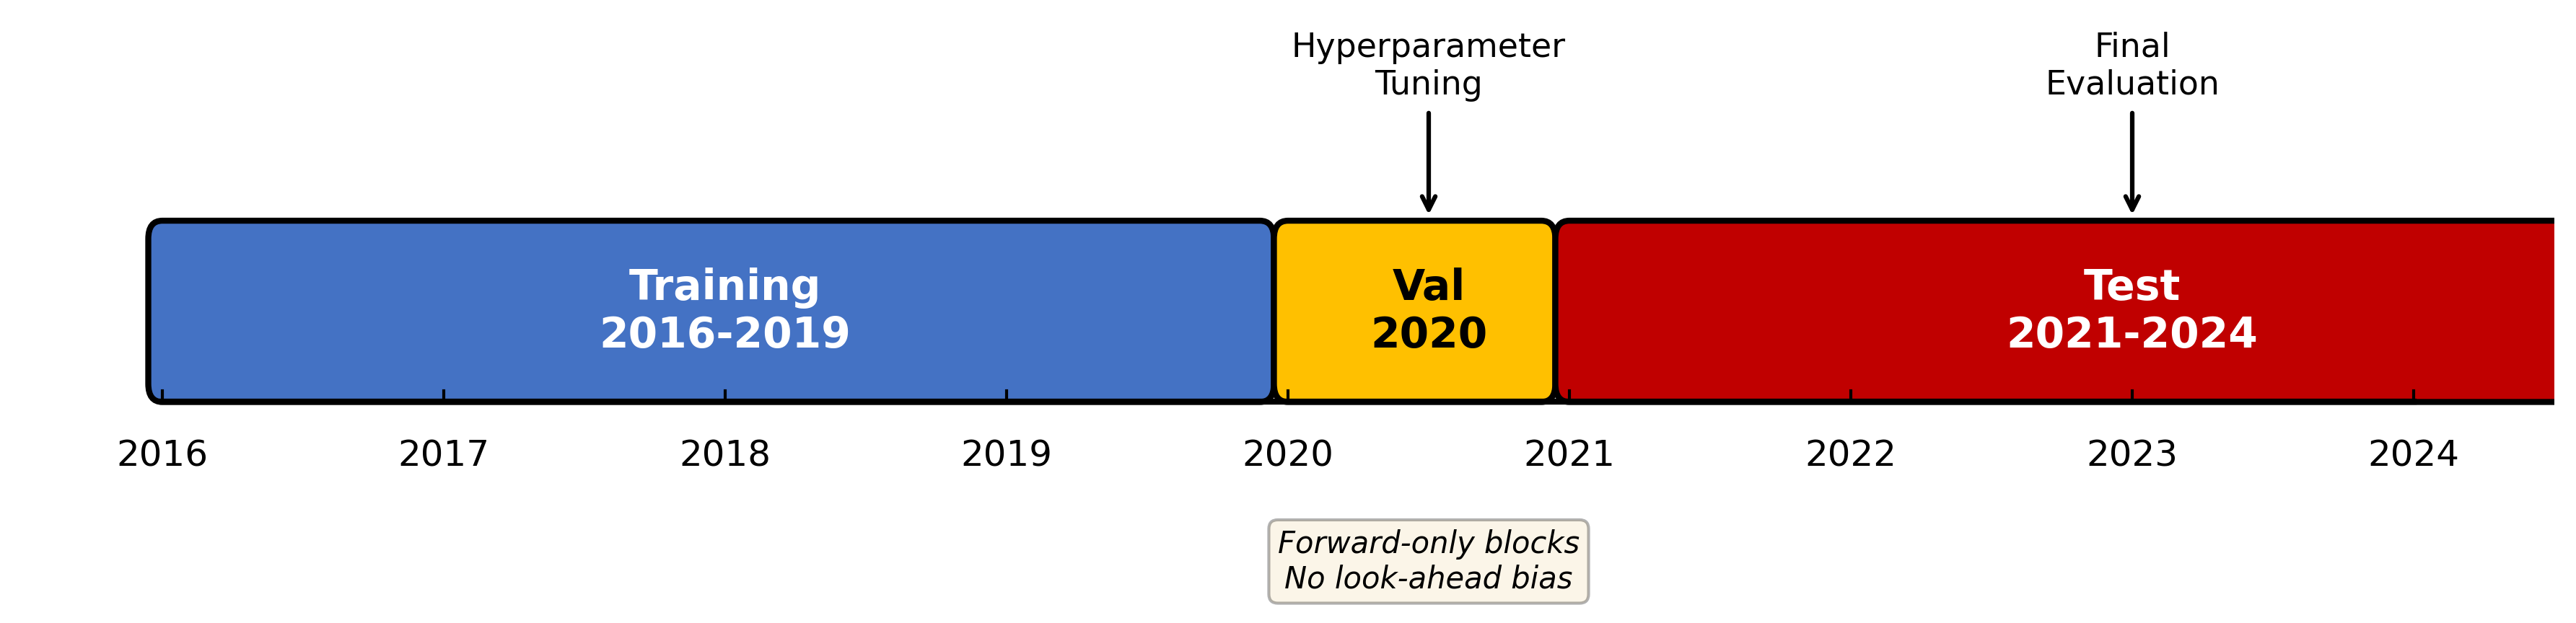
\includegraphics[width=0.9\textwidth]{figs/experiment_timeline.png}
  \end{center}
  
  \textbf{Data:} Dow 30 stocks (fixed as of 2018)\\[0.2cm]
  \textbf{Timeline:}
  \begin{itemize}
    \item \textcolor{blue}{Train:} 2016--2019 (4 years)
    \item \textcolor{orange}{Validation:} 2020 (COVID year, held out)
    \item \textcolor{red}{Test:} 2021--2024 (4 years, multiple regimes)
  \end{itemize}
  
  \vspace{0.3cm}
  
  \textbf{Horizons:} $h \in \{1, 5, 21\}$ trading days\\[0.2cm]
  \textbf{Target:} Log returns $r_{t\to t+h} = \ln(P_{t+h}) - \ln(P_t)$
\end{frame}

\begin{frame}{Data \& Features}
  \begin{columns}[T]
    \begin{column}{0.48\textwidth}
      \textbf{Feature Groups}
      
      \vspace{0.3cm}
      
      \textbf{1. Technical Indicators}
      \begin{itemize}
        \item Momentum (5, 10, 20 day)
        \item Moving averages
        \item Volatility (rolling std)
        \item RSI, MACD
        \item Volume features
      \end{itemize}
      
      \vspace{0.3cm}
      
      \textbf{2. Earnings Features}
      \begin{itemize}
        \item Earnings surprise \%
        \item Days to/from earnings
        \item Announcement flags
        \item Event windows ($\pm$3 days)
      \end{itemize}
    \end{column}
    
    \begin{column}{0.48\textwidth}
      \textbf{Data Sources}
      \begin{itemize}
        \item \textbf{Prices:} yfinance
        \item \textbf{Earnings:} API Ninjas
        \item \textbf{Macro:} FRED API
      \end{itemize}
      
      \vspace{0.5cm}
      
      \textbf{Leakage Controls}
      \begin{itemize}
        \item After-market data shifted to $t+1$
        \item Forward-only blocks
        \item 5-day embargos between splits
        \item Scaling fit on train only
        \item No look-ahead bias
      \end{itemize}
      
      \vspace{0.3cm}
      
      \textbf{Global Training}
      \begin{itemize}
        \item Pooled across all 30 stocks
        \item Shared parameters
      \end{itemize}
    \end{column}
  \end{columns}
\end{frame}

\begin{frame}{Models Tested}
  \small
  \begin{columns}[T]
    \begin{column}{0.45\textwidth}
      \textbf{Tabular Models}
      \begin{itemize}\scriptsize
        \item \textbf{Ridge Regression}
        \begin{itemize}
          \item Linear baseline
          \item L2 regularization
          \item $\alpha$ tuned on validation
        \end{itemize}
        
        \item \textbf{Random Forest}
        \begin{itemize}
          \item 100 trees, depth 5
          \item Strong tabular learner
        \end{itemize}
        
        \item \textbf{XGBoost}
        \begin{itemize}
          \item Gradient boosting
          \item Depth 3, lr 0.1
        \end{itemize}
      \end{itemize}
      
      \vspace{0.2cm}
      \scriptsize
      \textit{Trained separately per horizon}
    \end{column}
    
    \begin{column}{0.5\textwidth}
      \textbf{Sequence Models}
      \begin{itemize}\scriptsize
        \item \textbf{LSTM}
        \begin{itemize}
          \item 64 hidden, 1 layer
          \item 60-day lookback
          \item Multi-horizon output
        \end{itemize}
        
        \item \textbf{GRU}
        \begin{itemize}
          \item 64 hidden, 1 layer
          \item Simpler than LSTM
        \end{itemize}
        
        \item \textbf{TFT (Temporal Fusion Transformer)}
        \begin{itemize}
          \item 4 attn heads, 1 layer
          \item Hidden dim 16
          \item Multi-horizon output
          \item $\sim$50k parameters
        \end{itemize}
      \end{itemize}
      
      \vspace{0.2cm}
      \scriptsize
      \textit{Predict all horizons simultaneously}
    \end{column}
  \end{columns}
\end{frame}

\begin{frame}{TFT Architecture}
  \begin{center}
    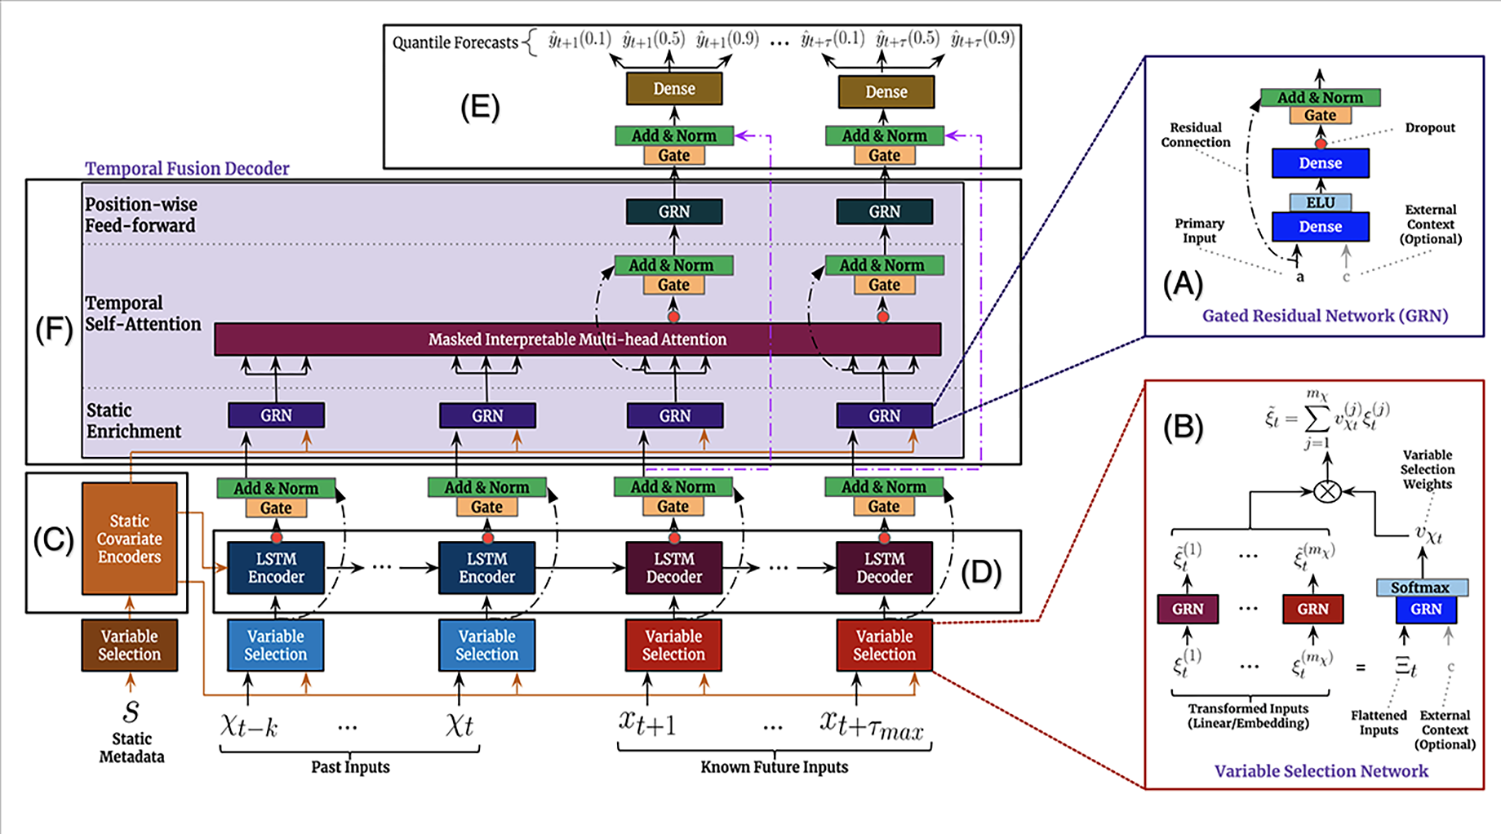
\includegraphics[width=0.65\textwidth]{figs/tft_architecture.png}
  \end{center}
  
  \vspace{0.2cm}
  
  \small
  \begin{itemize}
    \item \textbf{Static encoders:} Stock metadata
    \item \textbf{Historical encoders:} Past prices, technical indicators
    \item \textbf{Future encoders:} Known future covariates
    \item \textbf{Multi-head attention:} Learn temporal dependencies
    \item \textbf{Multi-horizon heads:} Predict $h\in\{1,5,21\}$ simultaneously
  \end{itemize}
\end{frame}

\begin{frame}{Evaluation Metrics}
  \scriptsize
  \textbf{Three complementary metrics:}
  
  \vspace{0.2cm}
  
  \begin{enumerate}
    \item \textbf{Root Mean Squared Error (RMSE)}
    \begin{itemize}\scriptsize
      \item Measures prediction precision in log-return units
    \end{itemize}
    
    \vspace{0.15cm}
    
    \item \textbf{Coefficient of Determination ($\rTwo$)}
    \begin{equation*}
      \rTwo = 1 - \frac{\sum_i {(y_i - \hat{y}_i)}^2}{\sum_i {y_i}^2}
    \end{equation*}
    \begin{itemize}\scriptsize
      \item vs.\ zero-return baseline
      \item Negative values common (low signal-to-noise)
    \end{itemize}
    
    \vspace{0.15cm}
    
    \item \textbf{Directional Accuracy (DA)}
    \begin{equation*}
      \da = \Pr[\text{sign}(\hat{r}) = \text{sign}(r)]
    \end{equation*}
    \begin{itemize}\scriptsize
      \item Most important for trading
      \item 50\% = random, >50\% = predictive
    \end{itemize}
  \end{enumerate}
\end{frame}

% ============================================
% SECTION 5: RESULTS
% ============================================
\section{Results}

\begin{frame}{Main Results: Performance by Horizon}
  \begin{center}
    \scriptsize
    \begin{tabular}{llccc}
      \toprule
      \textbf{Model} & \textbf{$h$} & \textbf{RMSE} & \textbf{$\rTwo$} & \textbf{DA} \\
      \midrule
      \multicolumn{5}{c}{\textit{$h=1$ (next day)}} \\
      \textbf{LSTM} & 1 & \textbf{0.0162} & -0.003 & \textbf{51.7\%} \\
      GRU & 1 & 0.0162 & -0.006 & 50.1\% \\
      \textbf{Rand. Forest} & 1 & 0.0164 & -0.023 & \textbf{51.9\%} \\
      Ridge & 1 & 0.0163 & -0.018 & 50.0\% \\
      \midrule
      \multicolumn{5}{c}{\textit{$h=5$ (one week)}} \\
      \textbf{Ridge} & 5 & \textbf{0.0365} & -0.020 & 51.2\% \\
      Rand. Forest & 5 & 0.0397 & -0.207 & 53.1\% \\
      \textbf{LSTM} & 5 & 0.0578 & -0.002 & \textbf{55.4\%} \\
      GRU & 5 & 0.0579 & -0.003 & 54.2\% \\
      \midrule
      \multicolumn{5}{c}{\textit{$h=21$ (one month)}} \\
      \textbf{LSTM} & 21 & \textbf{0.0508} & -0.002 & \textbf{55.0\%} \\
      GRU & 21 & 0.0509 & -0.002 & 53.9\% \\
      TFT & 21 & 0.0510 & -0.007 & 53.9\% \\
      Ridge & 21 & 0.0742 & -0.028 & 52.8\% \\
      \bottomrule
    \end{tabular}
  \end{center}
  
  \vspace{0.2cm}
  
  \begin{alertblock}{Key Takeaway}
    \small
    \textbf{LSTM} wins at $h=1$ \& $h=21$. \textbf{Ridge} dominates at $h=5$. TFT competitive but not superior.
  \end{alertblock}
\end{frame}

\begin{frame}{Directional Accuracy Across Horizons}
  \begin{center}
    \includegraphics[width=0.85\textwidth]{../comparison/artifacts/figures/fig1_da_by_horizon.png}
  \end{center}
  
  \vspace{0.3cm}
  
  \textbf{Key Observations:}
  \begin{itemize}
    \item Sequence models (LSTM/GRU) improve with horizon length
    \item Tabular models stay flat or degrade
    \item At $h=21$: LSTM reaches 55\%, vs. ~52\% for tabular baselines
    \item TFT competitive but not leading
  \end{itemize}
\end{frame}

\begin{frame}{Why Are All $\rTwo$ Values Negative?}
  \tiny
  \begin{block}{This is Normal in Finance!}
    \tiny
    $\rTwo$ vs.\ zero: $\rTwo = 1 - \frac{\sum (y_i - \hat{y}_i)^2}{\sum y_i^2}$
  \end{block}
  
  \vspace{0.15cm}
  
  \scriptsize
  \textbf{Interpretation:}
  \begin{itemize}\tiny
    \item Negative $\rTwo$ = worse than predicting zero
    \item Reflects market efficiency (low signal/noise)
    \item \textcolor{ForestGreen}{\textbf{LSTM (-0.002)}} better
    \item \textcolor{red}{\textbf{Rand. Forest (-0.248)}} overfitting
  \end{itemize}
  
  \vspace{0.15cm}
  
  \begin{alertblock}{Important}
    \tiny
    Despite negative $\rTwo$, \textbf{RMSE} and \textbf{DA} show meaningful differences. \textit{DA > 50\% economically significant.}
  \end{alertblock}
\end{frame}

\begin{frame}{Hypothesis 1: TFT Superiority?}
  \begin{block}{H1: Model Class Advantage}
    \textbf{Hypothesis:} TFT will outperform baselines at $h=21$\\
    \textbf{Criteria:} $\geq$2\,pp DA improvement or $\geq$5\% RMSE reduction
  \end{block}
  
  \vspace{0.5cm}
  
  \textbf{Results at $h=21$:}
  \begin{center}
    \begin{tabular}{lcc}
      \toprule
      \textbf{Model} & \textbf{RMSE} & \textbf{DA (\%)} \\
      \midrule
      LSTM & \textbf{0.05084} & \textbf{55.0} \\
      GRU & 0.05085 & 53.9 \\
      TFT & 0.05096 & 53.9 \\
      \bottomrule
    \end{tabular}
  \end{center}
  
  \vspace{0.5cm}
  
  \begin{alertblock}{Verdict: \textcolor{red}{\textbf{H1 NOT SUPPORTED}}}
    \scriptsize
    \begin{itemize}
      \item LSTM beats TFT by 0.24\% RMSE and 1.1\,pp DA
      \item Differences $<$ thresholds (2\,pp, 5\%)
      \item \textbf{Attention provides no advantage here}
    \end{itemize}
  \end{alertblock}
\end{frame}

\begin{frame}{Hypothesis 2: Earnings Features Matter?}
  \begin{columns}[T]
    \begin{column}{0.48\textwidth}
      \textbf{Ablation Study at $h=21$}
      
      \vspace{0.3cm}
      
      \small
      \begin{tabular}{lcc}
        \toprule
        \textbf{Features} & \textbf{RMSE} & \textbf{DA} \\
        \midrule
        \multicolumn{3}{c}{\textit{TFT}} \\
        Tech only & 0.0513 & 52.2\% \\
        Tech+Earnings & \textbf{0.0509} & \textbf{53.3\%} \\
        \midrule
        \multicolumn{3}{c}{\textit{XGBoost}} \\
        Tech only & 0.0817 & 51.1\% \\
        Tech+Earnings & \textbf{0.0812} & \textbf{51.8\%} \\
        \bottomrule
      \end{tabular}
      
      \vspace{0.5cm}
      
      \textbf{Overall improvement:}
      \begin{itemize}
        \item DA: +1.1\,pp
        \item RMSE: slightly better
      \end{itemize}
    \end{column}
    
    \begin{column}{0.48\textwidth}
      \textbf{Earnings Window Analysis}
      
      \vspace{0.3cm}
      
      \small
      \begin{tabular}{lcc}
        \toprule
        \textbf{Period} & \textbf{RMSE} & \textbf{DA} \\
        \midrule
        Earnings ($\pm$3d) & 0.0695 & \textbf{61.4\%} \\
        Non-earnings & 0.0666 & 53.9\% \\
        \bottomrule
      \end{tabular}
      
      \vspace{0.5cm}
      
      \textbf{During earnings windows:}
      \begin{itemize}
        \item \textcolor{ForestGreen}{+7.5\,pp improvement in DA!}
        \item Modest RMSE increase (higher volatility)
      \end{itemize}
    \end{column}
  \end{columns}
  
  \vspace{0.5cm}
  
  \begin{alertblock}{Verdict: \textcolor{ForestGreen}{\textbf{H2 SUPPORTED}}}
    Earnings features provide modest overall gains but \textbf{substantial improvements during announcement windows}. Confirms post-earnings-announcement drift.
  \end{alertblock}
\end{frame}

\begin{frame}{Hypothesis 3: Regime Dependence}
  \small
  \begin{columns}[T]
    \begin{column}{0.55\textwidth}
      \includegraphics[width=\textwidth]{../comparison/artifacts/figures/fig2_regime_rmse_heatmap.png}
      
      \vspace{0.2cm}
      
      \scriptsize
      Darker = lower RMSE (better)
    \end{column}
    
    \begin{column}{0.4\textwidth}
      \scriptsize
      \textbf{Best Models by Regime}
      
      \vspace{0.2cm}
      
      \begin{tabular}{lcc}
        \toprule
        \textbf{Regime} & \textbf{Best} & \textbf{RMSE} \\
        \midrule
        \multicolumn{3}{c}{\textit{Bear 2022}} \\
        & GRU & 0.0636 \\
        \midrule
        \multicolumn{3}{c}{\textit{Rally 2023--24}} \\
        & LSTM & 0.0475 \\
        \bottomrule
      \end{tabular}
      
      \vspace{0.3cm}
      
      \textbf{Directional Accuracy}
      \begin{itemize}
        \item Bear 2022: \textcolor{red}{All $<$50\%}
        \item Rally: \textcolor{ForestGreen}{56.2\%}
      \end{itemize}
    \end{column}
  \end{columns}
  
  \vspace{0.2cm}
  
  \begin{alertblock}{Verdict: \textcolor{ForestGreen}{\textbf{H3 SUPPORTED}}}
    \scriptsize
    Model rankings change across regimes. Sequence models excel in bull markets but \textbf{fail in bear markets}.
  \end{alertblock}
\end{frame}

% ============================================
% SECTION 6: DISCUSSION
% ============================================
\section{Discussion \& Insights}

\begin{frame}{Why Did Simple Models Win?}
  \small
  \begin{enumerate}
    \item \textbf{Data constraints}
    \begin{itemize}
      \item Small panel: 30 stocks, daily frequency
      \item Limited sample for deep learning; TFT's 50k params may be too many
    \end{itemize}
    
    \vspace{0.2cm}
    
    \item \textbf{Signal characteristics}
    \begin{itemize}
      \item Very low signal-to-noise ratio
      \item Short-term patterns quasi-linear (Ridge wins at $h=5$)
    \end{itemize}
    
    \vspace{0.2cm}
    
    \item \textbf{Model capacity trade-offs}
    \begin{itemize}
      \item More parameters $\Rightarrow$ harder training with weak signals
      \item LSTM/GRU ($\sim$25k) vs. TFT ($\sim$50k params)
      \item Simpler = better bias-variance trade-off
    \end{itemize}
    
    \vspace{0.2cm}
    
    \item \textbf{Feature engineering matters}
    \begin{itemize}
      \item Strong technical indicators capture most signal
      \item Tabular models exploit these effectively
    \end{itemize}
  \end{enumerate}
\end{frame}

\begin{frame}{When Do Transformers Shine?}
  \small
  \textbf{Our negative result for TFT suggests:}
  
  \vspace{0.3cm}
  
  \begin{block}{Transformers Need More}
    \small
    \begin{enumerate}
      \item \textbf{Larger datasets}
      \begin{itemize}\small
        \item TimesFM: trained on 100B time points
        \item Our study: $\sim$30 stocks $\times$ 8 years
      \end{itemize}
      
      \item \textbf{Richer modalities}
      \begin{itemize}\small
        \item Text: news, earnings calls, social media
        \item Alternative data: satellite, credit card
        \item BloombergGPT, FinGPT integrate multimodal data
      \end{itemize}
      
      \item \textbf{Longer horizons / higher frequency}
      \begin{itemize}\small
        \item Intraday: more samples; Long-term: clearer patterns
      \end{itemize}
      
      \item \textbf{Pretraining}
      \begin{itemize}\small
        \item Transfer learning; Foundation models for finance
      \end{itemize}
    \end{enumerate}
  \end{block}
\end{frame}

\begin{frame}{Practical Recommendations}
  \small
  \begin{block}{Model Selection by Horizon}
    \small
    \begin{itemize}
      \item \textbf{$h=1$ (daily):} LSTM or Random Forest
      \item \textbf{$h=5$ (weekly):} Ridge regression
      \item \textbf{$h=21$ (monthly):} LSTM or GRU
    \end{itemize}
  \end{block}
  
  \vspace{0.2cm}
  
  \begin{block}{When to Use Transformers}
    \small
    Only if you have:
    \begin{itemize}
      \item Large datasets (many stocks, long history)
      \item Multimodal inputs (text + prices)
      \item Computational resources
      \item Ability to leverage pretraining
    \end{itemize}
  \end{block}
  
  \vspace{0.2cm}
  
  \begin{block}{Feature Engineering Matters}
    \small
    \begin{itemize}
      \item Technical indicators capture most signal
      \item Earnings features add value near announcements
      \item Traditional feature engineering essential
    \end{itemize}
  \end{block}
\end{frame}

\begin{frame}{Economic Significance vs. Statistical Accuracy}
  \tiny
  \begin{alertblock}{Important Caveat}
    \tiny
    We focus on \textbf{statistical accuracy} (RMSE, $\rTwo$, DA), not \textbf{profitability}
  \end{alertblock}
  
  \vspace{0.15cm}
  
  \scriptsize
  \textbf{What we don't test:}
  \begin{itemize}\tiny
    \item Trading strategies, transaction costs
    \item Position sizing, risk management
    \item Sharpe ratio, maximum drawdown
  \end{itemize}
  
  \vspace{0.15cm}
  
  \begin{block}{Reality Check}
    \tiny
    \begin{itemize}
      \item 55\% directional accuracy \textit{might} be profitable
      \item Depends on: trading frequency, spreads, commissions
      \item Full backtesting needed for economic value
    \end{itemize}
  \end{block}
\end{frame}

\begin{frame}{Limitations}
  \small
  \begin{enumerate}
    \item \textbf{Limited universe}: Dow 30 only (large-cap U.S.)
    \begin{itemize}\small
      \item May not generalize to small-cap, international, or other assets
    \end{itemize}
    
    \item \textbf{Daily frequency only}
    \begin{itemize}\small
      \item Intraday patterns not explored
      \item Lower frequencies (weekly, monthly) not tested
    \end{itemize}
    
    \item \textbf{Hyperparameter tuning}
    \begin{itemize}\small
      \item Lightweight tuning on validation set; may favor simpler models
    \end{itemize}
    
    \item \textbf{Single split}
    \begin{itemize}\small
      \item Rolling/expanding window validation recommended for robustness
    \end{itemize}
    
    \item \textbf{Extreme events}
    \begin{itemize}\small
      \item Black swan events remain challenging for all pattern-based models
    \end{itemize}
  \end{enumerate}
\end{frame}

% ============================================
% SECTION 7: CONCLUSIONS
% ============================================
\section{Conclusions \& Future Work}

\begin{frame}{Key Findings Summary}
  \begin{enumerate}
    \item \textbf{Simple models match or beat transformers}
    \begin{itemize}
      \item LSTM best at $h=1$ and $h=21$
      \item Ridge best at $h=5$
      \item TFT competitive but not superior
    \end{itemize}
    
    \vspace{0.3cm}
    
    \item \textbf{Earnings features add value}
    \begin{itemize}
      \item +1.1\,pp overall DA improvement
      \item +7.5\,pp during earnings windows (61.4\% vs. 53.9\%)
      \item Confirms post-earnings-announcement drift
    \end{itemize}
    
    \vspace{0.3cm}
    
    \item \textbf{Performance is regime-dependent}
    \begin{itemize}
      \item GRU best in bear market (2022)
      \item LSTM best in bull market (2023--24)
      \item All models struggle in high-volatility downturns
    \end{itemize}
    
    \vspace{0.3cm}
    
    \item \textbf{Complexity is not always better}
    \begin{itemize}
      \item More parameters $\neq$ better performance
      \item Data constraints favor simpler models
      \item Feature engineering remains crucial
    \end{itemize}
  \end{enumerate}
\end{frame}

\begin{frame}{Contributions to the Field}
  \textbf{What makes this work valuable?}
  
  \vspace{0.5cm}
  
  \begin{enumerate}
    \item \textbf{Rigorous benchmarking}
    \begin{itemize}
      \item Apples-to-apples comparison across model classes
      \item Strict temporal validation (no look-ahead bias)
      \item Multiple random seeds for statistical reliability
    \end{itemize}
    
    \vspace{0.3cm}
    
    \item \textbf{Honest negative results}
    \begin{itemize}
      \item Transformers don't always win
      \item Important for setting realistic expectations
      \item Guides future research directions
    \end{itemize}
    
    \vspace{0.3cm}
    
    \item \textbf{Comprehensive evaluation}
    \begin{itemize}
      \item Multi-metric (RMSE, $\rTwo$, DA)
      \item Regime analysis
      \item Event window analysis
      \item Ablations
    \end{itemize}
    
    \vspace{0.3cm}
    
    \item \textbf{Baseline for future work}
    \begin{itemize}
      \item Researchers can compare against our results
      \item Code and methodology available
    \end{itemize}
  \end{enumerate}
\end{frame}

\begin{frame}{Future Directions}
  \small
  \begin{block}{1. Multi-Modal Integration}
    \small
    \begin{itemize}
      \item News, earnings transcripts, social media, macro text
      \item \textit{Hypothesis:} Transformers excel with heterogeneous data
    \end{itemize}
  \end{block}
  
  \vspace{0.2cm}
  
  \begin{block}{2. Alternative Data Sources}
    \small
    \begin{itemize}
      \item Satellite imagery, credit card data, web scraping, order flow
    \end{itemize}
  \end{block}
  
  \vspace{0.2cm}
  
  \begin{block}{3. Methodological Extensions}
    \small
    \begin{itemize}
      \item Larger universes (S\&P 500, Russell 3000)
      \item Intraday/high-frequency data; Longer horizons (quarterly, annual)
      \item Cross-asset learning (stocks, bonds, commodities)
    \end{itemize}
  \end{block}
\end{frame}

\begin{frame}{Future Work (Continued)}
  \small
  \begin{block}{4. Advanced Architectures}
    \small
    \begin{itemize}
      \item PatchTST, TimesFM-style pretraining, CNN+Transformer hybrids
      \item Graph neural networks for sector relationships
    \end{itemize}
  \end{block}
  
  \vspace{0.2cm}
  
  \begin{block}{5. Interpretability \& Explainability}
    \small
    \begin{itemize}
      \item Attention weights, feature importance (SHAP, LIME)
      \item Regime detection; Understanding when/why models fail
    \end{itemize}
  \end{block}
  
  \vspace{0.2cm}
  
  \begin{block}{6. Economic Evaluation}
    \small
    \begin{itemize}
      \item Full backtesting with transaction costs, portfolio optimization
      \item Risk-adjusted returns (Sharpe, Sortino), real-world deployment
    \end{itemize}
  \end{block}
\end{frame}

\begin{frame}{Take-Home Messages}
  \begin{alertblock}{For Practitioners}
    \begin{enumerate}
      \item Start simple: LSTM/Ridge can match transformers on daily data
      \item Don't neglect feature engineering
      \item Earnings events provide predictable opportunities
      \item Monitor regime changes carefully
      \item Always validate with strict temporal splits
    \end{enumerate}
  \end{alertblock}
  
  \vspace{0.5cm}
  
  \begin{alertblock}{For Researchers}
    \begin{enumerate}
      \item Transformers need scale: more data, richer modalities
      \item Negative results are valuable—publish them!
      \item Multi-modal integration is promising direction
      \item Benchmark against strong, well-tuned baselines
      \item Economic evaluation is crucial next step
    \end{enumerate}
  \end{alertblock}
\end{frame}

% ============================================
% THANK YOU / Q&A
% ============================================
\begin{frame}[plain]
  \centering
  \vspace{2cm}
  \Huge Thank You!
  
  \vspace{1cm}
  
  \Large Questions?
  
  \vspace{1.5cm}
  
  \normalsize
  \textbf{Contact:}\\[0.3cm]
  Nelson Siu\\
  \texttt{nelson.siu@mail.utoronto.ca}\\[0.5cm]
  
  Jonathan H. Chan\\
  \texttt{jonathan@sit.kmutt.ac.th}\\[0.8cm]
  
  \small
  \textit{Code and supplementary materials available upon request}
\end{frame}

% ============================================
% BACKUP SLIDES
% ============================================
\appendix

\begin{frame}{Backup: Detailed Performance Table}
  \tiny
  \begin{tabular}{llcccc}
    \toprule
    \textbf{Model} & \textbf{$h$} & \textbf{RMSE} & \textbf{$\rTwo$} & \textbf{DA} & \textbf{Std} \\
    \midrule
    GRU & 1 & 0.016249 & -0.006072 & 0.500920 & $\pm$0.024931 \\
    GRU & 5 & 0.057883 & -0.002885 & 0.542105 & $\pm$0.036308 \\
    GRU & 21 & 0.050854 & -0.002185 & 0.539142 & $\pm$0.033861 \\
    LSTM & 1 & 0.016222 & -0.002677 & 0.516688 & $\pm$0.015768 \\
    LSTM & 5 & 0.057849 & -0.001694 & 0.554207 & $\pm$0.018432 \\
    LSTM & 21 & 0.050840 & -0.001629 & 0.550429 & $\pm$0.021653 \\
    Random Forest & 1 & 0.016387 & -0.023148 & 0.519454 & $\pm$0.000290 \\
    Random Forest & 5 & 0.039717 & -0.206505 & 0.531379 & $\pm$0.000636 \\
    Random Forest & 21 & 0.081805 & -0.248432 & 0.542956 & $\pm$0.001095 \\
    Ridge & 1 & 0.016346 & -0.018058 & 0.500254 & $\pm$0.008734 \\
    Ridge & 5 & 0.036514 & -0.019737 & 0.511699 & $\pm$0.012456 \\
    Ridge & 21 & 0.074214 & -0.027501 & 0.528230 & $\pm$0.015892 \\
    TFT & 1 & 0.016453 & -0.031783 & 0.489379 & $\pm$0.019597 \\
    TFT & 5 & 0.057907 & -0.003690 & 0.550134 & $\pm$0.012030 \\
    TFT & 21 & 0.050963 & -0.006502 & 0.538742 & $\pm$0.029354 \\
    XGBoost & 1 & 0.016464 & -0.032850 & 0.515368 & $\pm$0.011245 \\
    XGBoost & 5 & 0.038217 & -0.117070 & 0.508611 & $\pm$0.014567 \\
    XGBoost & 21 & 0.081344 & -0.234415 & 0.516713 & $\pm$0.017234 \\
    \bottomrule
  \end{tabular}
\end{frame}

\begin{frame}{Backup: Hyperparameters}
  \small
  \begin{columns}[T]
    \begin{column}{0.48\textwidth}
      \textbf{Tabular Models}
      \begin{itemize}
        \item \textbf{Ridge:} $\alpha \approx 1.0$ (tuned on val)
        \item \textbf{Random Forest:}
        \begin{itemize}
          \item 100 trees
          \item Max depth: 5
          \item Min samples leaf: 1
        \end{itemize}
        \item \textbf{XGBoost:}
        \begin{itemize}
          \item Max depth: 3
          \item Learning rate: 0.1
          \item 100 rounds
        \end{itemize}
      \end{itemize}
    \end{column}
    
    \begin{column}{0.48\textwidth}
      \textbf{Sequence Models}
      \begin{itemize}
        \item \textbf{LSTM/GRU:}
        \begin{itemize}
          \item Hidden units: 64
          \item Layers: 1
          \item Dropout: 0.2
          \item Lookback: 60 days
          \item Learning rate: $1\times10^{-3}$
        \end{itemize}
        \item \textbf{TFT:}
        \begin{itemize}
          \item Attention heads: 4
          \item Layers: 1
          \item Hidden dim: 16
          \item Dropout: 0.3
          \item Learning rate: $3\times10^{-4}$
        \end{itemize}
      \end{itemize}
    \end{column}
  \end{columns}
  
  \vspace{0.5cm}
  
  \textbf{Training:} Adam/AdamW optimizer, batch size 256, up to 10 epochs with early stopping on validation set
\end{frame}

\begin{frame}{Backup: Compute Efficiency}
  \begin{center}
    \begin{tabular}{lcc}
      \toprule
      \textbf{Model} & \textbf{Parameters} & \textbf{Training Time} \\
      \midrule
      Ridge & $\sim$100 & $<$1 min \\
      Random Forest & $\sim$10k & $\sim$5 min \\
      XGBoost & $\sim$10k & $\sim$10 min \\
      LSTM & $\sim$25k & $\sim$1 hour \\
      GRU & $\sim$25k & $\sim$1 hour \\
      TFT & $\sim$50k & $\sim$2--3 hours \\
      \bottomrule
    \end{tabular}
  \end{center}
  
  \vspace{0.5cm}
  
  \textbf{Trade-offs:}
  \begin{itemize}
    \item Tabular models: fast, competitive accuracy
    \item Sequence models: moderate cost, best long-horizon performance
    \item Transformers: expensive, no clear advantage on this dataset
  \end{itemize}
  
  \vspace{0.3cm}
  
  \textbf{Practical implication:} For rapid deployment and iteration, simpler models are advantageous
\end{frame}

\end{document}
